\documentclass[10pt]{report}
\usepackage[utf8]{inputenc}
\usepackage{amsfonts}
\usepackage{amsmath}
\usepackage{amssymb}
\usepackage{commath}
\usepackage[ngerman]{babel}
\usepackage{enumitem}
\usepackage{booktabs}
\usepackage{longtable}
\usepackage{relsize}
\usepackage{pgfplots}
\usepackage{csvsimple}
\usepackage{pgfplotstable}
\usepackage{siunitx}
\usepackage{fancyhdr}
\usepackage{color}
\usepackage{float}

\setlength\parindent{0pt}

\setcounter{chapter}{3}

\pagestyle{fancy}
\fancyhf{}
\lhead{GPET Versuch 2}
\rhead{Tim Luchterhand, Paul Nykiel}
\cfoot{\thepage}

\author{Tim Luchterhand, Paul Nykiel}
\title{GPET Versuch 2}

\begin{document}
        \maketitle

        \section{Bestimmung des Innenwiderstandes einer Quelle}
        \textbf{Aufgabe:} Nehmen Sie die Strom-Spannungskennlinie der Batterie auf. Verwenden sie hierzu Messtabelle
        1 und tragen Sie die Messwerte in ein Diagramm ein. Schließen Sie das Spannungsmessgerät
        vor der Batterie an, damit Sie die Batterie nicht über einen längeren
        Zeitraum kurzschließen.
		
		\begin{figure}[H]
            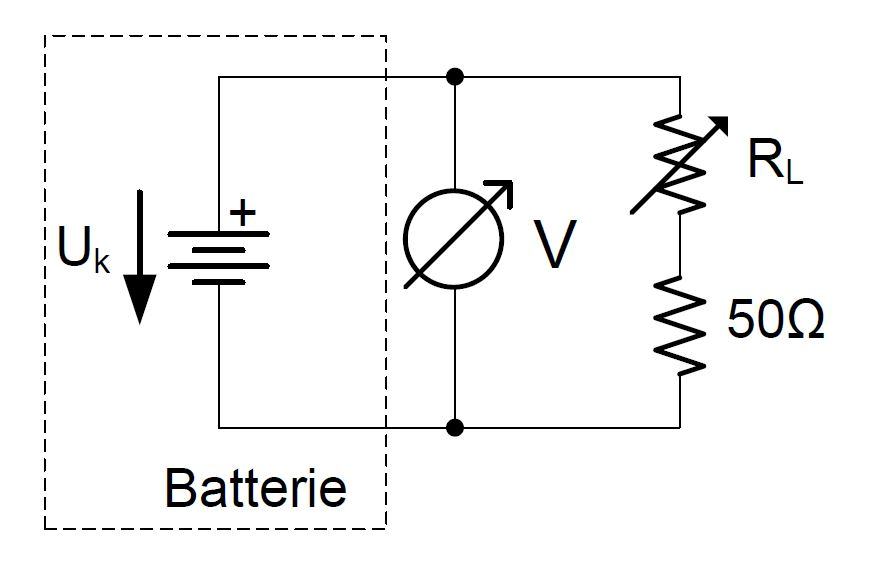
\includegraphics[width=\textwidth]{BatterieSchaltung.jpg}
          \caption{Schaltplan}
        \end{figure}

        \subsection{Vorgehensweise}
        Es werden verschiedene Lastwiderständer $R_L$ eingebaut und die Arbeitsgerade
        des Netzwerks aufgenommen. Der Laststrom $I_L$ berechnet sich aus
        \begin{equation*}
            I_L = \frac{U_{mess}}{R_L + 50\si{\ohm}}
        \end{equation*}


        \vspace{0.5cm}

        Der $0$-Wert bei $R_L$ repräsentiert einen Widerstand von $\infty \si{\ohm}$.
        \begin{table}[H]
            \begin{center}
                \caption{Messtabelle für Versuch 1}
                \label{tablec}
                \pgfplotstabletypeset[
                multicolumn names, % allows to have multicolumn names
                col sep=space, % the seperator in our .csv file
                display columns/0/.style={
                column name=$R_L$, % name of first column
                column type={S},string type},  % use siunitx for formatting
                display columns/1/.style={
                column name=$U_{mess}$,
                column type={S},string type},
                display columns/2/.style={
                column name=$I_L$,
                column type={S},string type},
                every head row/.style={
                before row={\toprule}, % have a rule at top
                after row={
                \si{\ohm} & \si{\volt} & m\si{\ampere}\\
                \midrule} % rule under units
                },
                every last row/.style={after row=\bottomrule},
                ]{quelleWiderstand.csv}
            \end{center}
        \end{table}

        \subsection{I-U-Kennlinie der Batterie}
        \begin{center}
            \begin{figure}[H]
              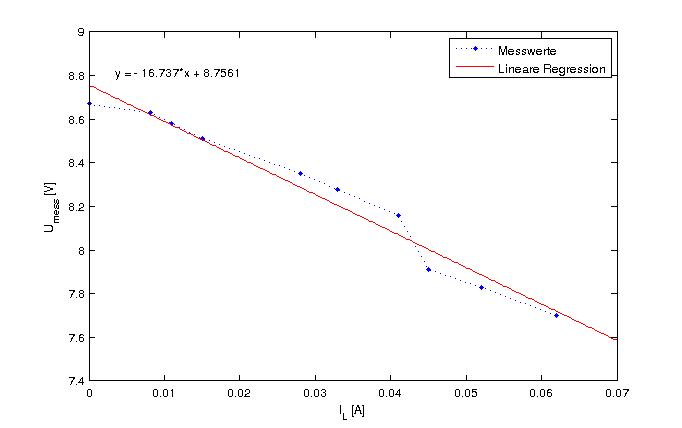
\includegraphics[width=\textwidth]{BatterieKurve.jpg}
              \caption{Arbeitsgerade}
            \end{figure}
        \end{center}

        \subsection{Charakterisierung der Ersatzspannungsquelle}
        \textbf{Aufgabe:} Charakterisieren Sie die Ersatzspannungsquelle mit Hilfe des erstellten Diagramms.

        \vspace{0.5cm}

        Die Steigung des Graphens ist der negative Innenwiderstand $R_{innen}$.
        Dieser beträgt:
        \begin{equation*}
            R_{innen} = 16.737 \si{\ohm}
        \end{equation*}

        Der x-Wert ($I$) des Schnittpunkts mit der x-Achse ist der Kurzschlussstrom.
        Dieser beträgt:
        \begin{equation*}
            I_{kurzschluss} = 0.523 \si{\ampere}
        \end{equation*}

        Der y-Wert ($U$) des Schnittpunkts mit der y-Achse ist die Leerlaufspannung.
        Diese beträgt:
        \begin{equation*}
            U_{leerlauf} = 8.75 \si{\volt}
        \end{equation*}

        \subsection{Messungenauigkeiten}
        Die Messungenauigkeit kommt durch das ungenaue Einstellen des Potetiometers
        und durch die Ungenauigekeit des Potentiometers selbst zustande. Weiterhin besitzt
		das Spannungsmessgerät eine Messungenauigkeit von ca. $1\%$ und man sollte von einem
		systematischen Fehler von $5\%$ ausgehen. Der linearer Verlauf der Kurve ist aber 
		trotzdem gut zu erkennen.


        \section{Untersuchung eines einfachen Netzwerks}
        \textbf{Aufgabe: }Bauen Sie die Schaltung aus Abbildung 6 nach. Die Widerstandswerte sind $R1 = R2 =
        1 \si{k\ohm}$ und $R3 = R4 = 100\si{\ohm}$.

        Bestimmen Sie die äquivalente Ersatzspannungsquelle zwischen den Knoten 0 und 1 durch
        Messung ($U_{in} = 3\si{\volt}$). Verwenden Sie hierzu wieder das Potentiometer mit $1\si{k\ohm}$ und tragen
        Sie die Ergebnisse in Messtabelle 2 ein.
		
		\begin{figure}[H]
            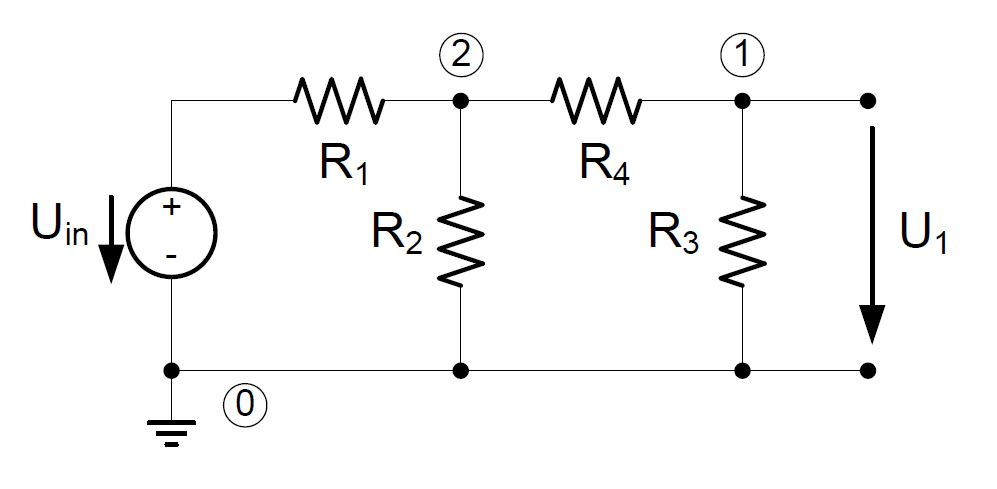
\includegraphics[width=\textwidth]{EinfachesNetzwerk.jpg}
          \caption{Schaltplan}
        \end{figure}

        \subsection{Vorgehensweise}
        Es werden verschiedene Lastwiderständer $R_L$ eingebaut und die Arbeitsgerade
        des Netzwerks aufgenommen. Der Laststrom $I_L$ berechnet sich aus
        \begin{equation*}
            I_L = \frac{U_{mess}}{R_L}
        \end{equation*}


        \vspace{0.5cm}

        Der $0$-Wert bei $R_L$ repräsentiert einen Widerstand von $\infty \si{\ohm}$.
        \begin{table}[H]
            \begin{center}
                \caption{Messtabelle für Versuch 2}
                \label{tableb}
                \pgfplotstabletypeset[
                multicolumn names, % allows to have multicolumn names
                col sep=space, % the seperator in our .csv file
                display columns/0/.style={
                column name=$R_L$, % name of first column
                column type={S},string type},  % use siunitx for formatting
                display columns/1/.style={
                column name=$U_{mess}$,
                column type={S},string type},
                display columns/2/.style={
                column name=$I_L$,
                column type={S},string type},
                every head row/.style={
                before row={\toprule}, % have a rule at top
                after row={
                \si{\ohm} & m\si{\volt} & m\si{\ampere}\\
                \midrule} % rule under units
                },
                every last row/.style={after row=\bottomrule},
                ]{einfachesNetzwerk.csv}
            \end{center}
        \end{table}

        \subsection{Ersatzspannungsquelle}
        \subsubsection{I-U-Kennlinie des Netzwerks}
        \begin{center}
            \begin{figure}[H]
              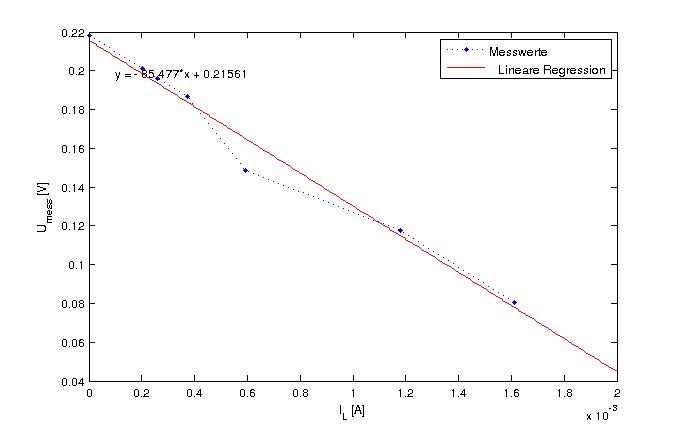
\includegraphics[width=\textwidth]{ErsatzspannungsQuelle.jpg}
              \caption{Arbeitsgerade}
            \end{figure}
        \end{center}

        Durch identisches Vorgehen zu Aufgabe 3.1 ergibt sich folgende
        Charakterisierung:
        \begin{eqnarray*}
            U_{Quelle} &=& 0.2156\si{\volt}\\
            I_{Kurzschluss} &=& 2.1\si{m\ampere}\\
            R_{Innen} &=& 85.477\si{\ohm}
        \end{eqnarray*}
		
		\vspace{0.5cm}
		
		Die gemessenen Werte stimmen mit den berechneten überein.


        \subsubsection{Messungenauigkeit}
        Die Messungenauigkeit kommt durch das ungenaue Einstellen des Potetiometers
        und durch die Ungenauigekeit des Potentiometers selbst zustande. Weiterhin besitzt
		das Spannungsmessgerät eine Messungenauigkeit von ca. $1\%$ und man sollte von einem
		systematischen Fehler von $5\%$ ausgehen. Der linearer Verlauf der Kurve ist aber 
		trotzdem gut zu erkennen.


        \subsection{Spannungen an den Widerständen}
        \textbf{Aufgabe:} Messen Sie die Spannungen an den Widerständen in Abhängigkeit von $U_{in}$. Tragen Sie
        die Messwerten in Messtabelle 3 ein und vergleichen diese mit den berechneten Werten in
        einem Diagramm.
        \begin{table}[H]
            \begin{center}
                \caption{Messtabelle für Versuch 2}
                \label{tablec}
                \pgfplotstabletypeset[
                multicolumn names, % allows to have multicolumn names
                col sep=space, % the seperator in our .csv file
                display columns/0/.style={
                column name=$U_{in}$, % name of first column
                column type={S},string type},  % use siunitx for formatting
                display columns/1/.style={
                column name=$U_{R1,soll}$,
                column type={S},string type},
                display columns/2/.style={
                column name=$U_{R2,soll}$,
                column type={S},string type},
                display columns/3/.style={
                column name=$U_{R3,soll}$,
                column type={S},string type},
                display columns/4/.style={
                column name=$U_{R4,soll}$,
                column type={S},string type},
                display columns/5/.style={
                column name=$U_{R1,mess}$,
                column type={S},string type},
                display columns/6/.style={
                column name=$U_{R2,mess}$,
                column type={S},string type},
                display columns/7/.style={
                column name=$U_{R3,mess}$,
                column type={S},string type},
                display columns/8/.style={
                column name=$U_{R4,mess}$,
                column type={S},string type},
                every head row/.style={
                before row={\toprule}, % have a rule at top
                after row={
                \si{\volt} & \si{\volt} & \si{\volt} & \si{\volt} & \si{\volt} & \si{\volt} & \si{\volt} & \si{\volt} & \si{\volt}\\
                \midrule} % rule under units
                },
                every last row/.style={after row=\bottomrule},
                ]{quelleWiderstand2.csv}
            \end{center}
        \end{table}

        \subsection{Diagramm}
        Berechnete Werte in \textcolor{red}{rot}, gemessene Werte in \textcolor{blue}{blau}.
        \subsubsection{Vergleich $R_1$}
        \begin{center}
            \begin{tikzpicture}
        		\begin{axis}[ymin=0, xmin=0, xlabel = {$U_{in}$[V]}, ylabel = {$U_{R_1}$[V]}]
        			\addplot[color=red] table[x index = {0},
                            y index = {1}] {quelleWiderstand2.csv};
                    \addplot[color=blue, only marks] table[x index = {0},
                            y index = {5}] {quelleWiderstand2.csv};
        		\end{axis}
        	\end{tikzpicture}
        \end{center}
        \subsubsection{Vergleich $R_2$}
        \begin{center}
            \begin{tikzpicture}
                \begin{axis}[ymin=0, xmin=0, xlabel = {$U_{in}$[V]}, ylabel = {$U_{R_2}$[V]}]
        			\addplot[color=red] table[x index = {0},
                            y index = {2}] {quelleWiderstand2.csv};
                    \addplot[color=blue, only marks] table[x index = {0},
                            y index = {6}] {quelleWiderstand2.csv};
        		\end{axis}
        	\end{tikzpicture}
        \end{center}
        \subsubsection{Vergleich $R_3$}
        \begin{center}
            \begin{tikzpicture}
                \begin{axis}[ymin=0, xmin=0, xlabel = {$U_{in}$[V]}, ylabel = {$U_{R_3}$[V]}]
        			\addplot[color=red] table[x index = {0},
                            y index = {3}] {quelleWiderstand2.csv};
                    \addplot[color=blue, only marks] table[x index = {0},
                            y index = {7}] {quelleWiderstand2.csv};
        		\end{axis}
        	\end{tikzpicture}
        \end{center}
        \subsubsection{Vergleich $R_4$}
        \begin{center}
            \begin{tikzpicture}
                \begin{axis}[ymin=0, xmin=0, xlabel = {$U_{in}$[V]}, ylabel = {$U_{R_4}$[V]}]
        			\addplot[color=red] table[x index = {0},
                            y index = {4}] {quelleWiderstand2.csv};
                    \addplot[color=blue, only marks] table[x index = {0},
                            y index = {8}] {quelleWiderstand2.csv};
        		\end{axis}
        	\end{tikzpicture}
        \end{center}


        \subsubsection{Messungenauigkeiten}
        Wie in den Diagrammem zu erkennen ist, weichen die Messwerte nur sehr
        gering von den berechneten Werten ab.

        Es ergibt es sich für jeden Widerstand eine charakteristische Gerade.
		Die kleinen Fehler rühren von einer gewissen Ungenauigkeit des Spannungsmessgeräts,
		sowie einem systematischen Fehler her.

        \section{Untersuchung eines komplizierten Netzwerks}
        \textbf{Aufgabe:} Messen Sie die Spannungen an allen
        Knoten in Abhängigkeit von $U_{in,1} = 0 \ldots 3 \si{\volt}$ und tragen Sie die Ergebnisse in Messtabelle
        4 ein. Erstellen Sie ein Diagramm für die Spannungen an allen Knoten in Abhängigkeit
        der Spannung $U_{in,1} = 0 \ldots 3 \si{\volt}$.
		
		\begin{figure}[H]
            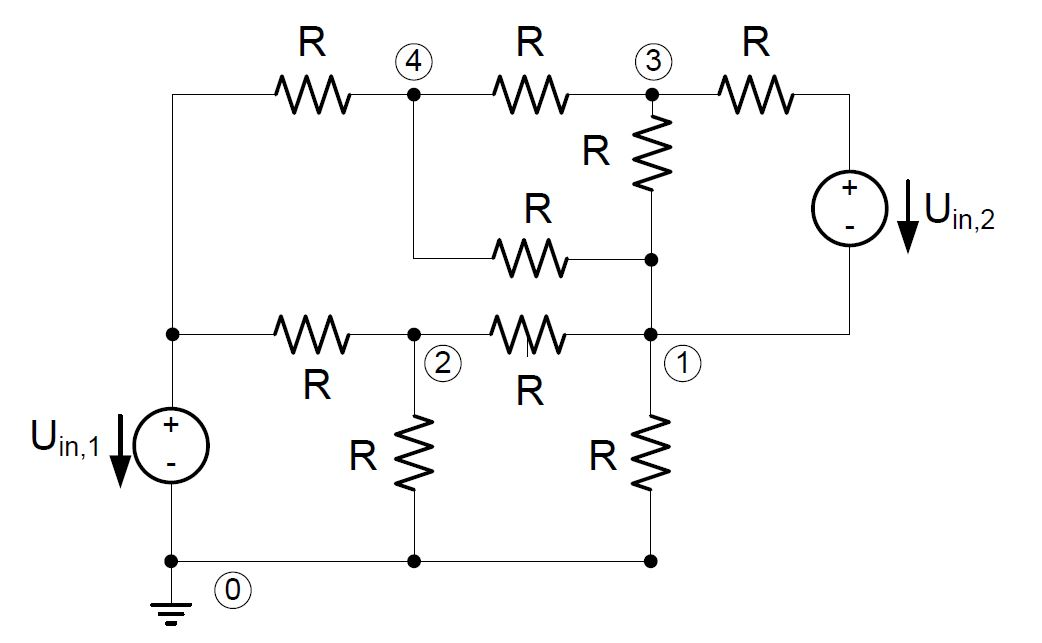
\includegraphics[width=\textwidth]{KomplexesNetzwerk.jpg}
          \caption{Schaltplan}
        \end{figure}
		
        \begin{table}[H]
            \begin{center}
                \caption{Messtabelle für Versuch 3}
                \label{tablec}
                \pgfplotstabletypeset[
                multicolumn names, % allows to have multicolumn names
                col sep=space, % the seperator in our .csv file
                display columns/0/.style={
                column name=$U_{in,1}$, % name of first column
                column type={S},string type},  % use siunitx for formatting
                display columns/1/.style={
                column name=$U_{1,mess}$,
                column type={S},string type},
                display columns/2/.style={
                column name=$U_{2,mess}$,
                column type={S},string type},
                display columns/3/.style={
                column name=$U_{3,mess}$,
                column type={S},string type},
                display columns/4/.style={
                column name=$U_{4,mess}$,
                column type={S},string type},
                every head row/.style={
                before row={\toprule}, % have a rule at top
                after row={
                \si{\volt} & \si{\volt} & \si{\volt} & \si{\volt} & \si{\volt}\\
                \midrule} % rule under units
                },
                every last row/.style={after row=\bottomrule},
                ]{kompliziertesNetzwerk.csv}
            \end{center}
        \end{table}

        \subsection{Diagramm der Knotenspannungen}
        $U_1$ in \textcolor{black}{schwarz}.

        $U_2$ in \textcolor{green}{grün}.

        $U_3$ in \textcolor{blue}{blau}.

        $U_4$ in \textcolor{red}{rot}.
        \begin{center}
            \begin{figure}[H]
                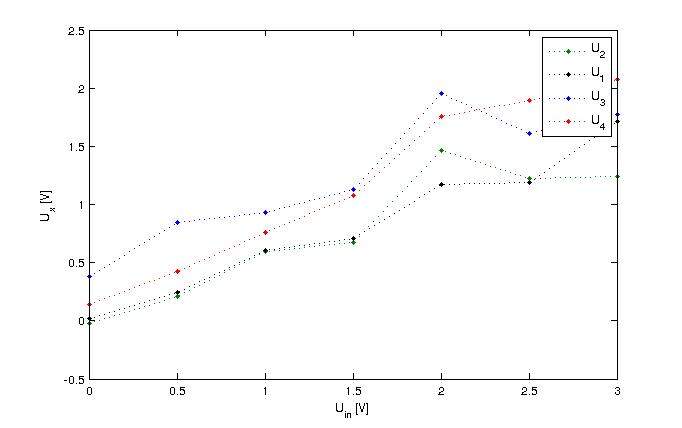
\includegraphics[width=\textwidth]{KPVmess.jpg}
              \caption{Messwerte}
            \end{figure}
        \end{center}

		//@TODO Diagramm mit linReg einfügen
		
        \subsubsection{Messungenauigkeiten}
        Wie im Diagramm zu erkennen, verhalten sich die Kurven zwar generell linear,
        besitzen aber markante Abweichungen. Während des Versuchs ist aufgefallen,
        dass durch Wackeln an den Kabeln der Messgeräte sich die Messwerte
        signifikant beeinflussen ließen. Die Sprünge im Diagramm lassen sich
        also auf den mangelhaften Zustand der Kabel zurückführen. Wir haben einige,
        jedoch nicht alle Messungen wiederholen können. Zum Teil gab es stark
        unterschiedliche Ergebnisse bei ein und der selben Messung.


        \subsection{Knotenpotenzialanalyse mit Matlab}
        \textbf{Aufgabe:} Nun soll für dieses Netzwerk das in Abschnitt 2.2 aufgestellte KPV mit Hilfe von Matlab
        gelöst und mit den Ergebnissen der eben durchgeführten Messungen verglichen werden.

        \vspace{0.5cm}

        \subsubsection{Matrix}
        \begin{equation*}
            \begin{bmatrix}
                -5G & G & 2G & G\\
                G & -3G & 0 & 0\\
                2G & 0 & -3G & G\\
                G & 0 & G & -3G
            \end{bmatrix}
            \begin{bmatrix}
                \varphi_1 \\
                \varphi_2 \\
                \varphi_3 \\
                \varphi_4
            \end{bmatrix}
            =
            \begin{bmatrix}
                I_3\\
                -I_2\\
                -I_3\\
                -I_1
            \end{bmatrix}
        \end{equation*}

        \subsubsection{Lösung}

        \begin{figure}[H]
            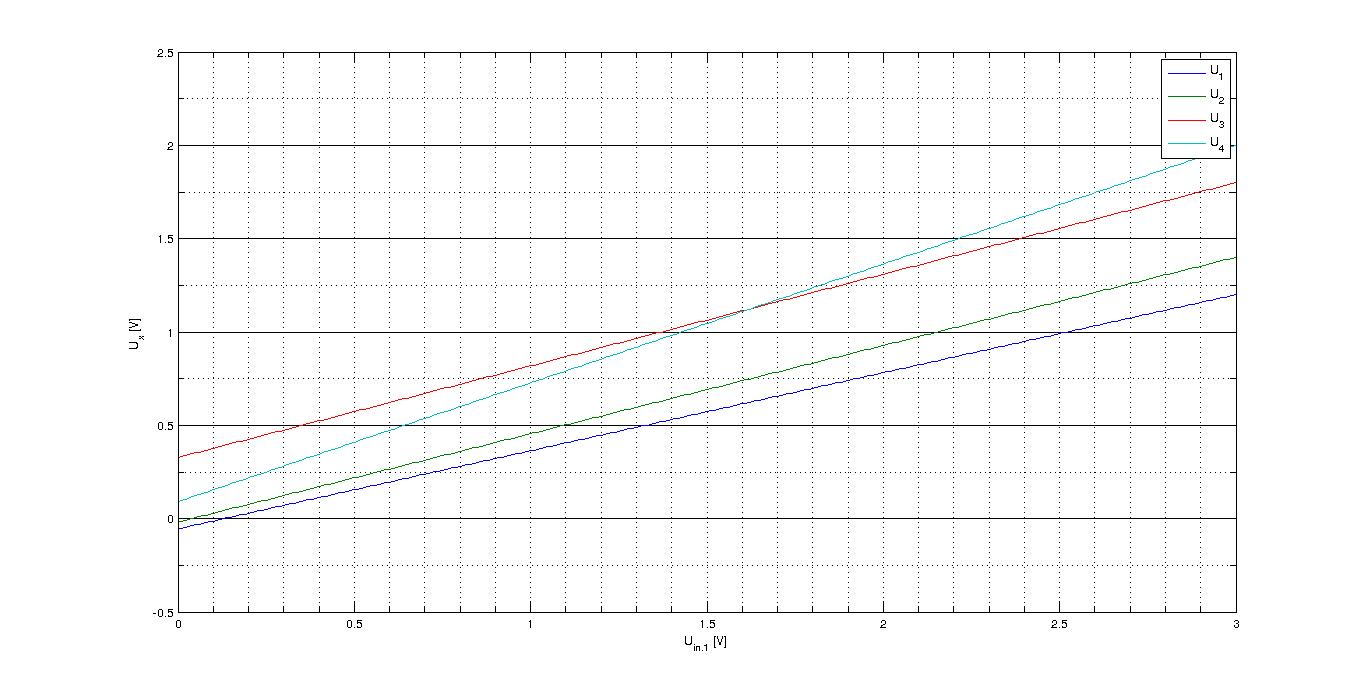
\includegraphics[width=\textwidth]{KPV.jpg}
          \caption{KPV\_plot mit MatLab}
        \end{figure}

        \subsubsection{Auswertung}
        Alle vier Potentiale Verhalten sich Linear. Die Steigung der Geraden
        repräsentiert das Spannungsteilerverhältniss zwischen $U_{in}$ und des
        jeweiligen Potentials $U_x$. Da die Spannungsteilerverhältnisse jeweils
		unterschiedlich sind, besitzen die Geraden auch jeweils unterschiedliche
		Steigungen.

        Beim Schnittpunkt zwischen $U_3$ und $U_4$ (bei ca.$1.6$V) befinden sich
        beide Knoten auf dem selben Potential, d.h.\ es fließt kein Strom zwischen
        ihnen.

        Das Offset der jeweiligen Kurven bei $U_{in} = 0$V kommt durch die zweite
        Spannungsquelle im Netzwerk, die eine konstanten Spannung von $1$V liefert,
        zustande. Da die Knoten 1 und 2 am –Pol von $U_{in2}$ angeschlossen sind, misst 
		man mit $U_{in1} = 0$V hier ein negatives Potential, während $U_3$ und $U_4$ auf
		einem positiven Potential liegen.

        \vspace{0.5cm}
		%@TODO Diagrammnummer einfügen
        Das Diagramm für die Messwerte verhält sich leider auf den ersten Blick nicht so,
		wie das berechnete. Durch die bereits oben geschilderten Messfehler und Probleme,
		sind zum Teil deutliche Sprünge und Abweichungen vom linearen Verlauf zu erkennen.
		In Diagramm NR? wurden die Messwerte durch Geraden angenähert. Hier ist nun, wie
		im berechneten Bild, der Schnittpunkt zwischen $U_3$ und $U_4$ gut zu erkennen, wenn auch
		etwas nach rechts verschoben (bei ca. $1.8$V). Ein weiterer  Schnittpunkt zwischen $U_1$
		uns $U_2$, der im berechneten Diagramm nicht zu sehen ist, ist ebenfalls den Messfehlern
		geschuldet.


        \section{Aufbau einer Messbrücke nach Wheatstone}
        \textbf{Aufgabe:} Kann mit diesem Messaufbau jeder Widerstand gemessen werden? Falls dies nicht der
        Fall ist, wie muss der Messaufbau verändert werden, damit die restlichen Widerstände
        gemessen werden können?

		\begin{figure}[H]
            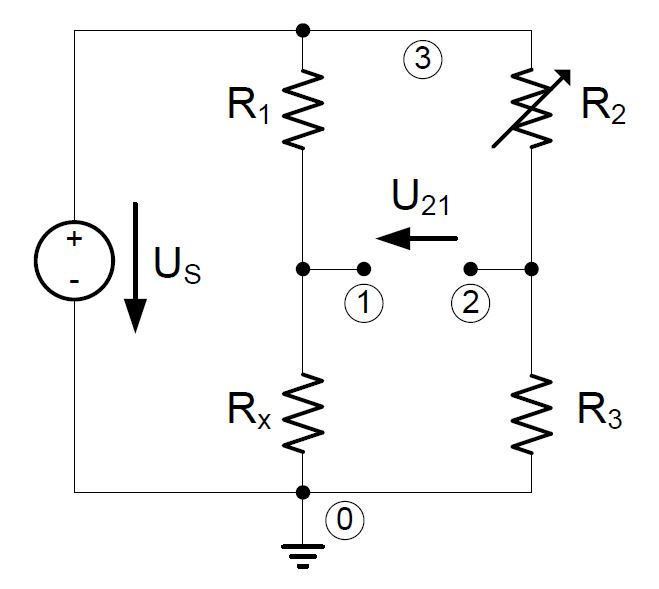
\includegraphics[width=\textwidth]{Wheatstone.jpg}
          \caption{Messbrücke nach Wheatstone}
        \end{figure}
		
        \subsection{Vorgehensweise}
        Der Widerstand des Potentiometers wird so lange verändert, bis die Spannung
        zwischen beiden Spannungsteilern genau null Volt beträgt. Der gesuchte
        Widerstand $R_x$ lässt sich dann wie folgt berechnen:

        \begin{equation*}
            R_x = \frac{R_1 R_3}{R_{poti}}
        \end{equation*}

        \vspace{0.5cm}

        Verwendet wurden folgende Widerstände:
        \begin{eqnarray*}
            R_1 &=& 100\si{\ohm}\\
            R_3 &=& 1\si{k\ohm}
        \end{eqnarray*}

        \subsection{Widerstand 1}
        \begin{eqnarray*}
            R_{poti} &=& 146.5 \si{\ohm} \\
            \Rightarrow R_{x} &=& 682.6 \si{\ohm}\\
            R_{mitMultimeter} &=& 678\si{\ohm} \\
			R_{tatsächlich} &=& 680\si{\ohm}\\
			\rho_{Wheatstone} &=& 0.30\%
        \end{eqnarray*}

        \subsection{Widerstand 2}
        \begin{eqnarray*}
            R_{poti} &=& 452.6 \si{\ohm} \\
            \Rightarrow R_{x} &=& 220.9\si{\ohm}\\
            R_{mitMultimeter} &=& 219.7\si{\ohm}\\
			R_{tatsächlich} &=& 220\si{\ohm}\\
			\rho_{Wheatstone} &=& 0.41\%
        \end{eqnarray*}

        \subsection{Widerstand 3}
        \begin{eqnarray*}
            R_{poti} &=& 211.8 \si{\ohm} \\
            \Rightarrow R_{x} &=& 472.1\si{\ohm}\\
            R_{mitMultimeter} &=& 469.0\si{\ohm}\\
			R_{tatsächlich} &=& 470\si{\ohm}\\
			\rho_{Wheatstone} &=& 0.45\%
        \end{eqnarray*}

		\subsubsection{Messungenauigkeiten}
        Der relative Fehler der Messung nach Wheatstone zum offiziellen Widerstandswert
		ist verschwindend gering. Der Fehler kommt durch die Ungenauigekeit des Spannungsmessgeräts,
		des Potetiometers und durch die Abweichung des Widerstands an sich zustande.
		
        \subsection{Einschränkungen}
        $R_1$, $R_2$ und $R_3$ müssen so gewählt werden, dass $I_L$ auch tatsächlich
        auf $0$A gebracht werden kann.

        \vspace{0.5cm}

        Ist $R_x$ beispielsweise zu groß für die gewählten Widerstände $R_1$ und $R_3$, muss
        man mit dem Potentiometer sehr kleine Widerstandswerte einstellen was zu
        Messungenauigkeiten führen kann.

        Es sollte gelten:
        \begin{equation*}
            \frac{R_1 \cdot R_3}{R_x} >> 1
        \end{equation*}
        damit mit dem Potentiometer keine kleinen Widerstände eingestellt werden
        müssen.

        Außerdem sollte $R_1$ in der Größenordnung von $R_x$ sein, damit auf der
        rechten Seite ein Spannungsteiler aus zwei großen Widerständen ist und auf
        der linken Seite vergleichsweise dazu zwei kleine Widerstände. Dadurch
        muss das Potentiometer auf einen großen Wert eingestellt werden und
        Messungenauigkeiten fallen nicht so sehr ins Gewicht.

\end{document}
